\section{Results analysis}

\subsection{What you Will Learn}

In this final part of the tutorial, you will learn how to analyse in detail the calculated particle field and compare it to the single-phase field, and to compare the numerical and experimental results using the particle output file that you set-up in the \textit{cs\_user\_postprocess.c} user functions.

\subsection{Verifying the Simulation}\label{lag:verify}

During the Lagrangian calculation, a ‘listla’ file is automatically created by \CS containing the data listed in \tablename~\ref{lag:listla}:

\begin{table}[H]
\begin{center}
\begin{tabular}{c l}
\Mline
\bf \ \ \ \ \ Column \ \ \ \ \  & \bf Description  \\
\hline\hline
1 & Number of the time step  \\
2 & Lagrangian physical time \\
3 & The number of instantaneous particles in the domain \\
4 & The number of instantaneous particles in the domain (with weighting) \\
5 & The number of particles injected in the domain \\
6 & The number of particles injected in the domain (with weight) \\
\multirow{2}{*}{7} & Instantaneous number of particles leaving the domain, \\
 & or deposed and eliminated \\
\multirow{2}{*}{8} & Instantaneous number of particles leaving the domain, \\
 & sticking to the wall and eliminated(with weighting) \\
9 & Instantaneous number of particles sticking to the wall \\
10 & Instantaneous number of particles sticking to walls (with weighting) \\
11 & Instantaneous number of particles lost \\
\Mline
\end{tabular}
\caption{Description of the data in the ‘listla’ file..\label{lag:listla}}
\end{center}
\end{table}

This information can be used to evaluate the convergence of the simulations.

For example, \figurename~\ref{lag:nb_particles} and \figurename~\ref{lag:particles_leaving} present, respectively, the number of particles in the domain and the number of particles entering and leaving the domain during the Lagrangian simulation.  It can be seen that both the number of particles in the domain and the number of particles leaving the domain is well established and remains stable after less than 200 time steps. The earlier decision, when setting up the Lagrangian model, of starting the particle statistical analysis at the $500^{th}$ time step is validated by this analysis.
%
\begin{figure}[H]
\centering
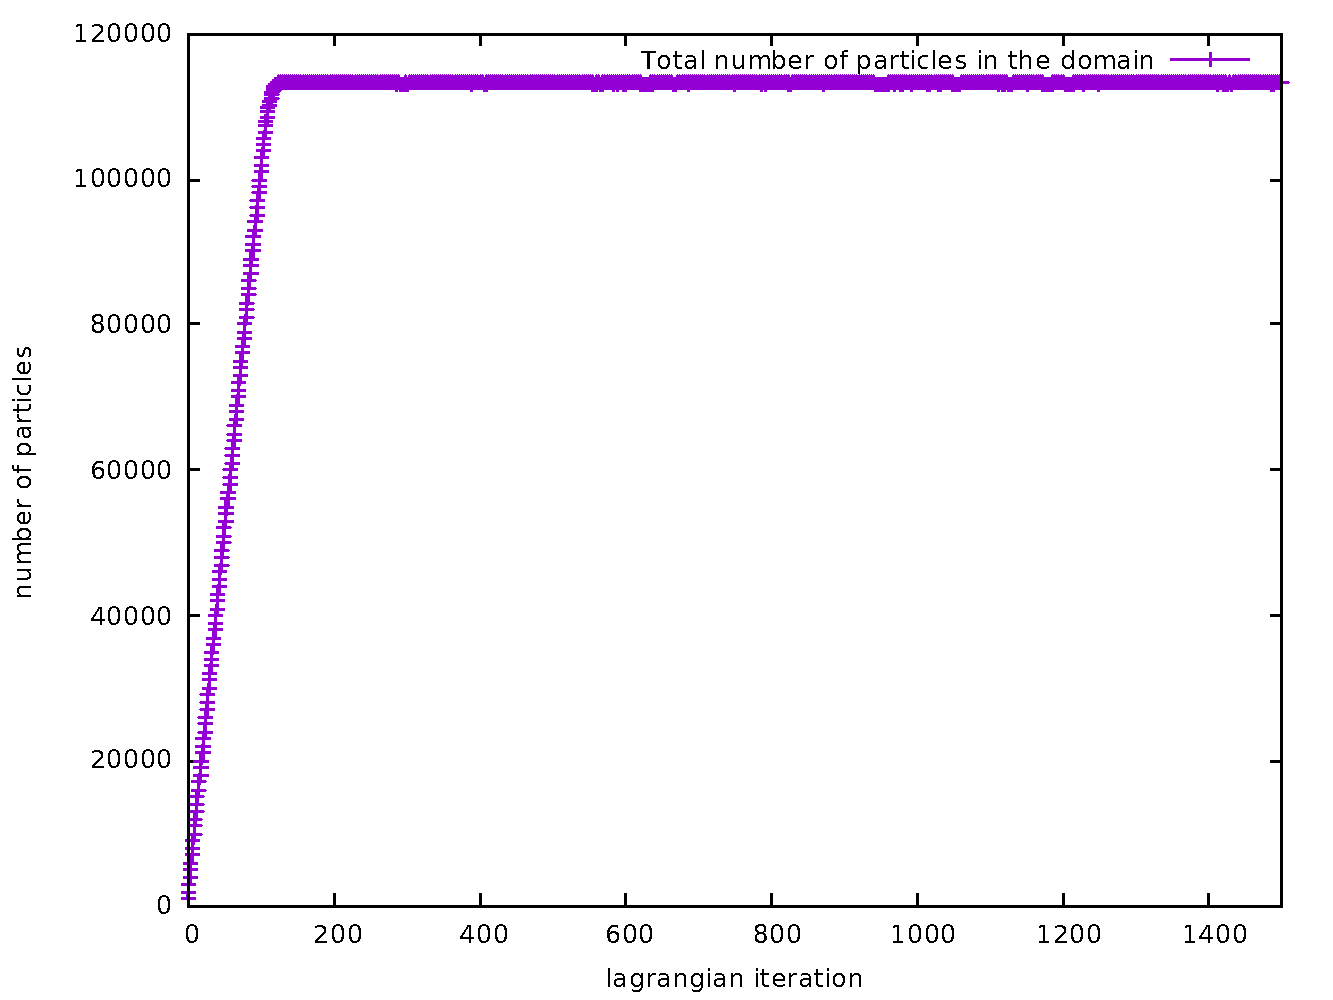
\includegraphics[width=0.7\textwidth]{\IMAGES/Part6_Results/particles_domain.pdf}
\caption{Number of particles in the computational domain over the first 1500 lagrangian iterations.}\label{lag:nb_particles}
\end{figure}
%
\begin{figure}[H]
\centering
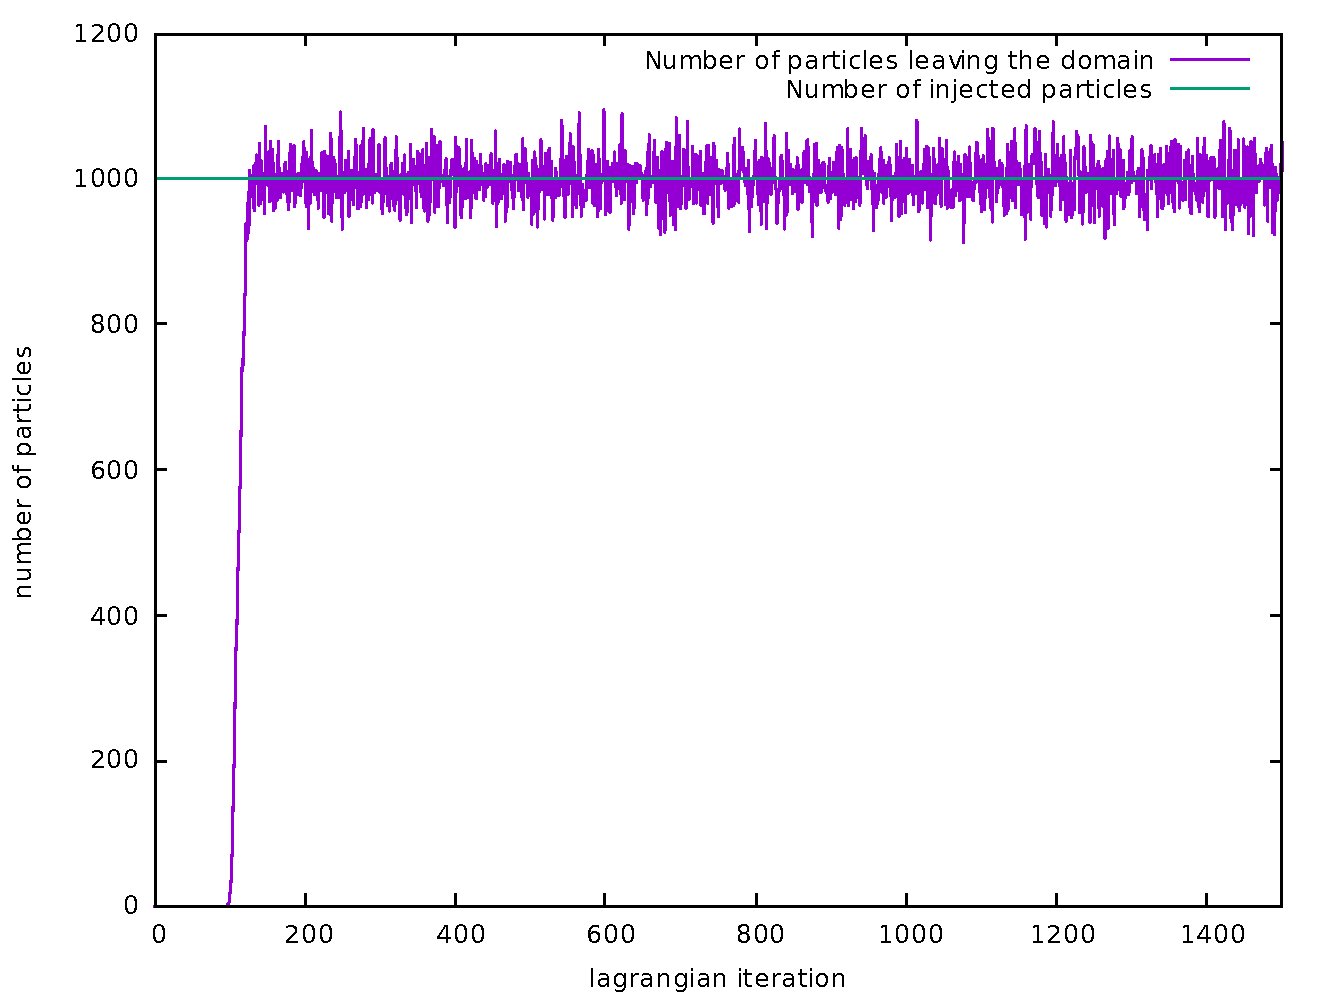
\includegraphics[width=0.7\textwidth]{\IMAGES/Part6_Results/particles_in_out.pdf}
\caption{Number of particles entering and leaving the computational domain over the first 1500 lagrangian iterations.}\label{lag:particles_leaving}
\end{figure}
%
\subsection{Flow Field}\label{lag:Resu_flow_field}

Starting with the analysis of the flow field in \paravis, \figurename~\ref{lag:part_vol_frac} presents a countour plot of the particle volume fraction in a 2D plane along the centre line of the pipe.  It can be seen that the majority of the particles injected into the flow domain remain along or near the pipe axis before spreading in spanwise direction.
%
\begin{figure}[H]
\centering
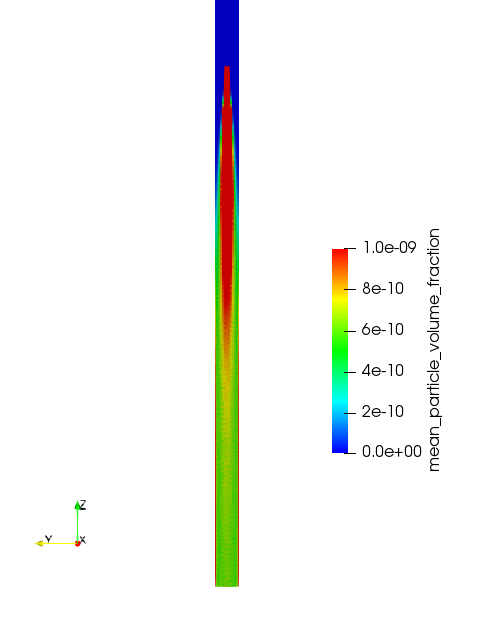
\includegraphics[width=0.8\textwidth]{\IMAGES/Part6_Results/lagr_part_vol_frac_crop.png}
\caption{Volume fraction of the particles in the pipe.}\label{lag:part_vol_frac}
\end{figure}
%
\figurename~\ref{lag:v_z} presents the $V_z$ velocity component of the carrier fluid, the vertical velocity of the particles and the $V_z$ velocity variance of these particles, also on 2D slices in the yz plane along the pipe centre line.
%
\begin{figure}[H]
\begin{subfigure}{0.3\textwidth}
\centering
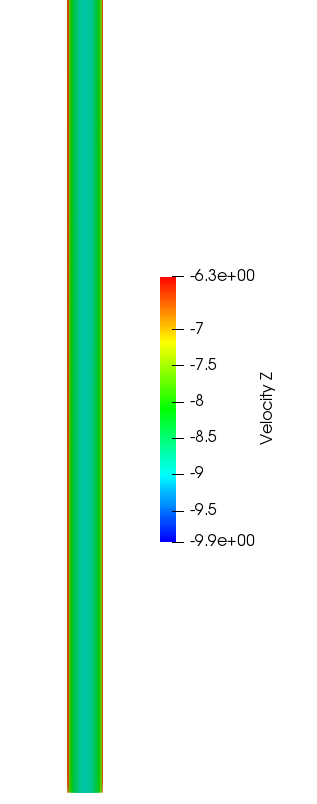
\includegraphics[width=\textwidth]{\IMAGES/Part6_Results/lagr_vel_z_crop.png}
\caption{$V_z$ velocity of the fluid\\ \ \ }
\label{lag:cap1_vel}
\end{subfigure}
\begin{subfigure}{0.3\textwidth}
\centering
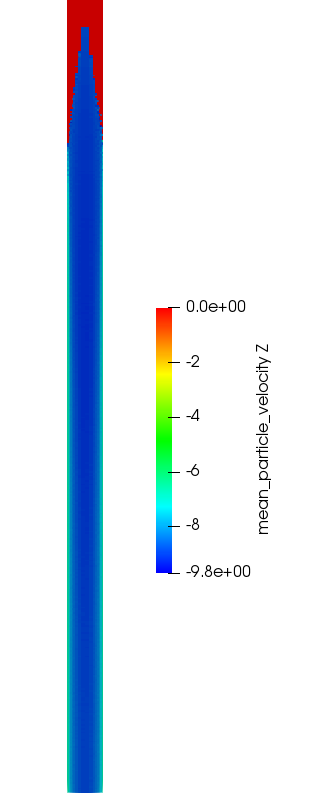
\includegraphics[width=\textwidth]{\IMAGES/Part6_Results/lagr_part_vel_z_crop.png}
\caption{$V_z$ velocity of the particles\\ \ \ }
\label{lag:cap2_vel}
\end{subfigure}
\begin{subfigure}{0.3\textwidth}
\centering
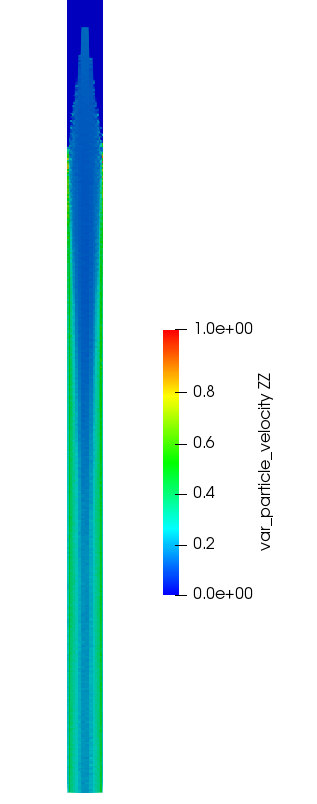
\includegraphics[width=\textwidth]{\IMAGES/Part6_Results/lagr_var_part_vel_z_crop.png}
\caption{Variance of the $V_z$ velocity of the particles}
\label{lag:cap3_vel}
\end{subfigure}
\caption{Visualization in the yz plane along the pipe axis}
\label{lag:v_z}
\end{figure}
%
It can be seen that, as the particles are very small, they are entrained by the fluid at the fluid velocity, with both the carrier fluid and the particles achieving a maximum velocity of the order of -9.5m/s, \figurename~\ref{lag:cap1_vel} and \figurename~\ref{lag:cap2_vel}.

The particle response and flow time scales may be compared to verify that, in this instance, the particles are expected to closely follow the carrier fluid.   For this low particle-Reynolds number flow, the relaxation time, $\tau_p$, of the particle is given by:

\begin{equation}
\tau _p \approx \dfrac{\rho_pd_p^2}{18\mu}=1.92\times10^{-4}s
\end{equation}

For turbulent dispersion, the flow time scale may be estimated as the characteristic time of the turbulence,$\tau^t_{12}$, calculated at the injection point:

\begin{equation}
\tau^t_{12}=\dfrac{3}{2}C_\mu\dfrac{k^2}{\epsilon}=2.726\times10^{-3}s
\end{equation}

Therefore,$\frac{\tau_p}{\tau^t_{12}}\ll1.0$, which confirms that the particles will follow the carrier fluid turbulence.

The variance of the vertical velocity of the particles (\figurename~\ref{lag:cap3_vel}) can be seen to be at a minimum along the pipe axis and at its highest close to the flow domain wall, due to the near wall effects such as the boundary layer and the particle rebound condition.

\subsection{Comparison of Predicted and Experimental Data}

The numerical and experimental data can be compared using the output data files 'Z318.csv', 'Z502.csv', 'Z679.csv', 'Z132.csv' which \CS wrote at the end of the calculation as a result of the programming in \textit{cs\_user\_postprocess.c} (\ref{lag:cs_user_postprocess.c}).

These files contain the particle normalised axial velocity, the particle concentration and the particle radial velocity at the $z = 0,318$, $z = 0,502$, $z = 0,679$ and $z = 1,32m$ planes where experimental data is also available. For convenience, the experimental data at these locations has been reproduced in Appendix \ref{lag:appendixA} from \cite{Arnason}.

\figurename~\ref{lag:z0318} to \figurename~\ref{lag:z132} present the predicted (green line) and measured (red symbols) data at the different measuring planes. The figures show that the calculated values of the axial velocity and  particle concentration are in rather good agreement with the experimental data for all measurement planes.  The radial component of the velocity is also in good agreement with the experiment data, except for z = 1.32m.  As the radial velocity decreases with the distance from the injection point and the concentration of particles near the walls increases, the error in the numerical results increases.

\begin{figure}[H]
\begin{subfigure}{0.33\textwidth}
\centering
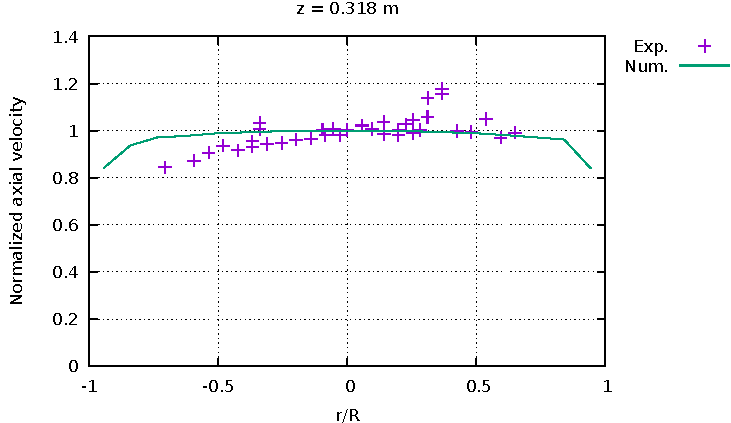
\includegraphics[width=\textwidth]{\IMAGES/Part6_Results/axial_z0318.pdf}
\caption{Axial velocity}\label{lag:axial_z0318}
\end{subfigure}
\begin{subfigure}{0.33\textwidth}
\centering
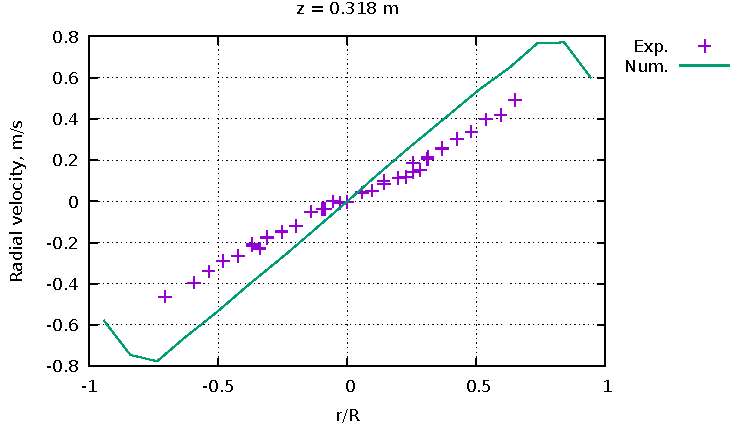
\includegraphics[width=\textwidth]{\IMAGES/Part6_Results/radial_z0318.pdf}
\caption{Radial velocity}\label{lag:radial_z0318}
\end{subfigure}
\begin{subfigure}{0.33\textwidth}
\centering
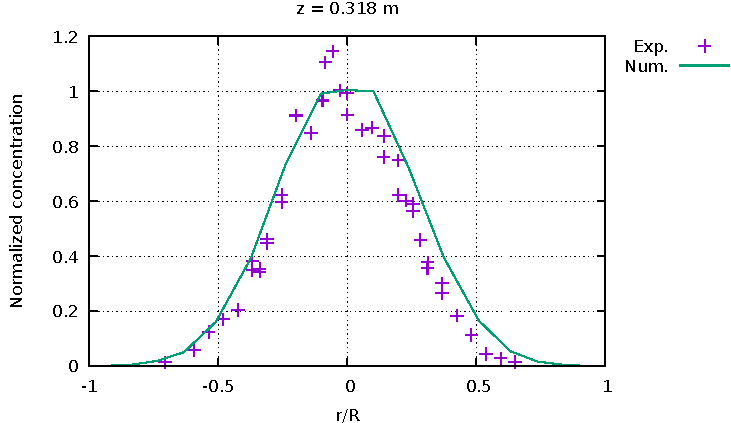
\includegraphics[width=\textwidth]{\IMAGES/Part6_Results/concentration_z0318.pdf}
\caption{Particle concentration}\label{lag:conc_z0318}
\end{subfigure}
\captionsetup{justification=centering}
\caption{Numerical (line) and experimental\cite{Arnason} (symbols) results at z = 0.318m.}
\label{lag:z0318}
\end{figure}

\begin{figure}[H]
\begin{subfigure}{0.33\textwidth}
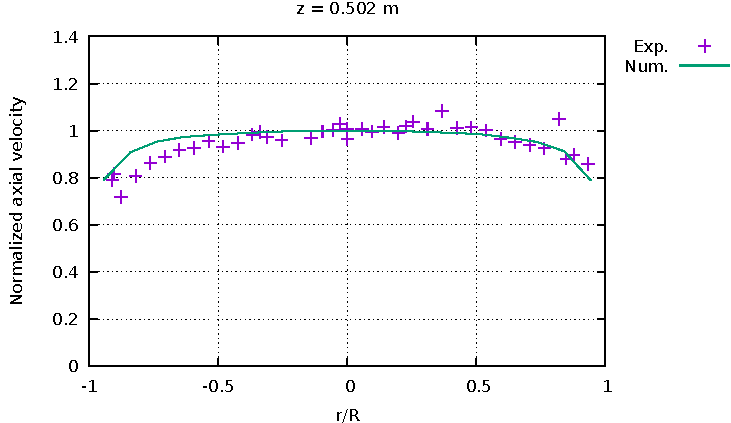
\includegraphics[width=\textwidth]{\IMAGES/Part6_Results/axial_z0502.pdf}
\caption{Axial velocity.}\label{lag:axial_z0502}
\end{subfigure}
\begin{subfigure}{0.33\textwidth}
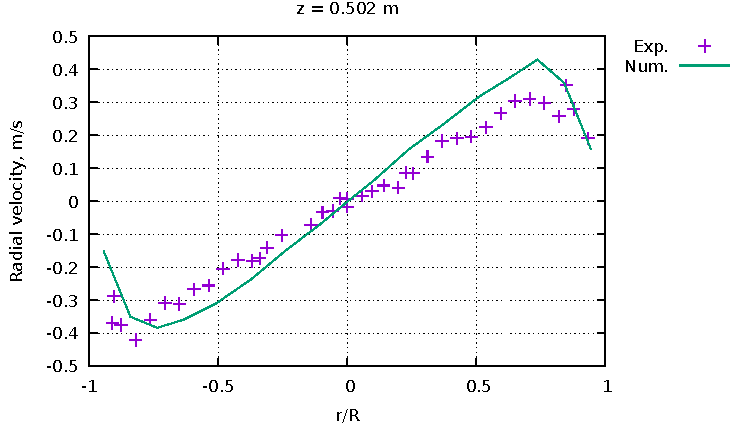
\includegraphics[width=\textwidth]{\IMAGES/Part6_Results/radial_z0502.pdf}
\caption{Radial velocity.}\label{lag:radial_z0502}
\end{subfigure}
\begin{subfigure}{0.33\textwidth}
\centering
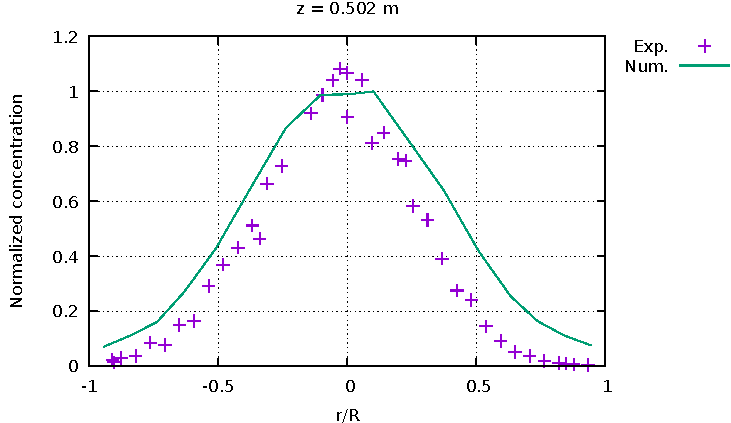
\includegraphics[width=\textwidth]{\IMAGES/Part6_Results/concentration_z0502.pdf}
\caption{Particle concentration}\label{lag:conc_z0502}
\end{subfigure}
\captionsetup{justification=centering}
\caption{Numerical (line) and experimental\cite{Arnason} (symbols) results at z = 0.502m.}
\label{lag:z0502}
\end{figure}

\begin{figure}[H]
\begin{subfigure}{0.33\textwidth}
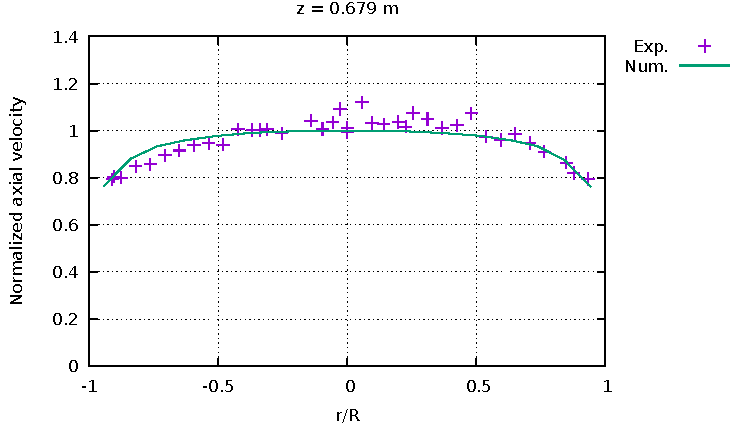
\includegraphics[width=\textwidth]{\IMAGES/Part6_Results/axial_z0679.pdf}
\caption{Axial velocity.}\label{lag:axial_z0679}
\end{subfigure}
\begin{subfigure}{0.33\textwidth}
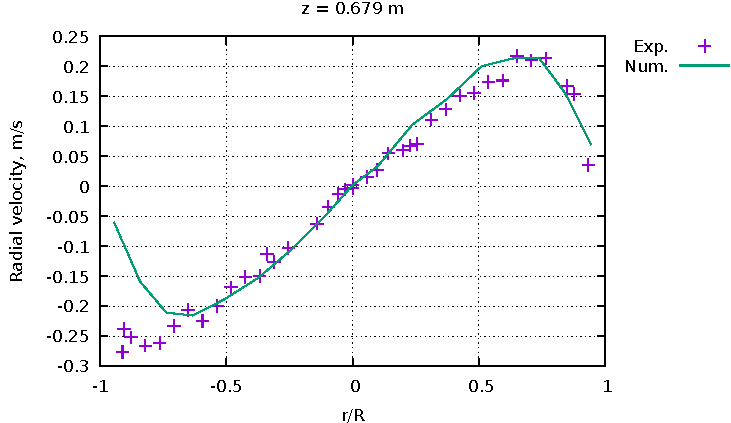
\includegraphics[width=\textwidth]{\IMAGES/Part6_Results/radial_z0679.pdf}
\caption{Radial velocity.}\label{lag:radial_z0679}
\end{subfigure}
\begin{subfigure}{0.33\textwidth}
\centering
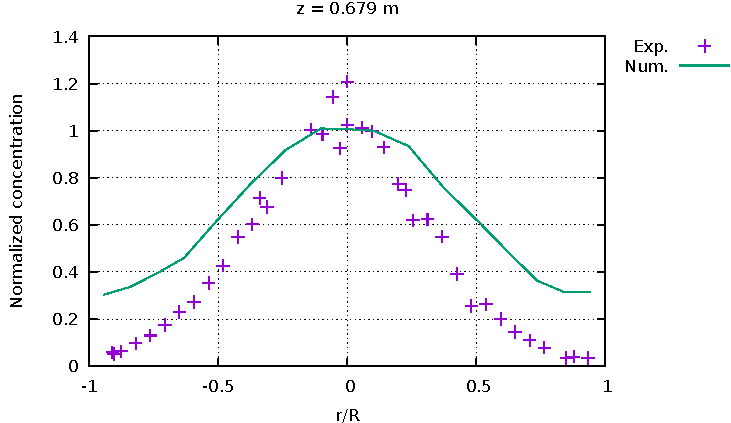
\includegraphics[width=\textwidth]{\IMAGES/Part6_Results/concentration_z0679.pdf}
\caption{Particle concentration}\label{lag:conc_z0679}
\end{subfigure}
\captionsetup{justification=centering}
\caption{Numerical (line) and experimental\cite{Arnason} (symbols) results at z = 0.679m.}
\label{lag:z0679}
\end{figure}

\begin{figure}[H]
\begin{subfigure}{0.33\textwidth}
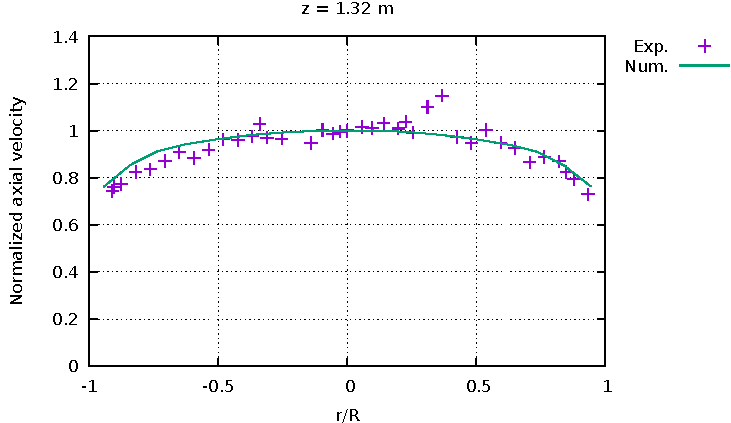
\includegraphics[width=\textwidth]{\IMAGES/Part6_Results/axial_z132.pdf}
\caption{Axial velocity.}\label{lag:axial_z132}
\end{subfigure}
\begin{subfigure}{0.33\textwidth}
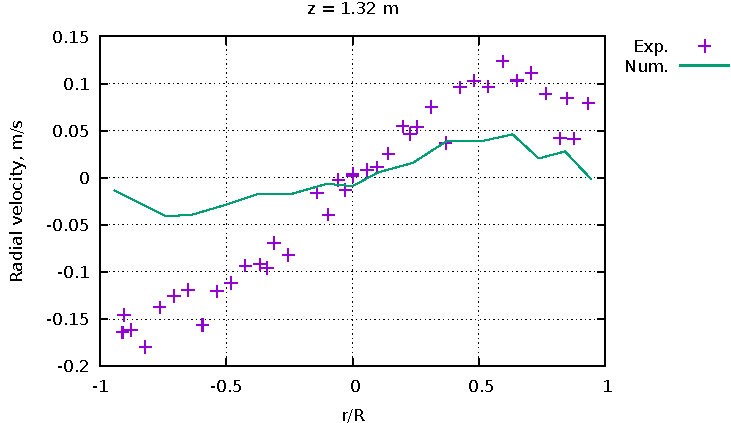
\includegraphics[width=\textwidth]{\IMAGES/Part6_Results/radial_z132.pdf}
\caption{Radial velocity.}\label{lag:radial_z132}
\end{subfigure}
\begin{subfigure}{0.33\textwidth}
\centering
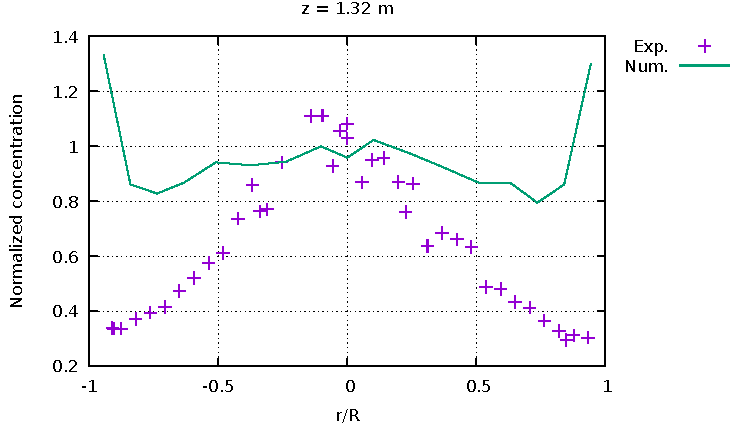
\includegraphics[width=\textwidth]{\IMAGES/Part6_Results/concentration_z132.pdf}
\caption{Particle concentration}\label{lag:conc_z132}
\end{subfigure}
\captionsetup{justification=centering}
\caption{Numerical (line) and experimental\cite{Arnason} (symbols) results at z = 1.32m.}
\label{lag:z132}
\end{figure}
